% ---- Don't modify from Line no. 2 to 74 ----
\documentclass[12pt]{article}

\usepackage{lineno,hyperref}
\modulolinenumbers[5]
\usepackage{graphics}
\usepackage{graphicx}
\usepackage{cite}
\usepackage{epsfig}
\usepackage{amsmath}   
\usepackage{amssymb}
\usepackage{placeins}
\usepackage[linesnumbered,ruled,vlined]{algorithm2e}
\usepackage{setspace}
\usepackage{multirow}
\usepackage[export]{adjustbox}[2011/08/13]
\usepackage{tabularx}
\usepackage{algcompatible}
\usepackage{caption}
\usepackage{epsf}
\usepackage{epstopdf}
\usepackage{subfigure} 
\usepackage{colortbl}
\usepackage{longtable}
\usepackage{enumerate}
\usepackage{tabularx, booktabs}

\usepackage[table,xcdraw]{xcolor}

\usepackage{tikz}
\usepackage{multirow}
\usepackage{enumitem}
\usepackage{soul}
\usepackage{xcolor}
\usepackage[utf8]{inputenc}
\usepackage{placeins}
\usepackage{makecell}
\newcounter{qcounter}
\usepackage{tcolorbox}
\usepackage{lscape}
\usepackage{url}
\usepackage{hyperref}
\usepackage{tablefootnote}
\usepackage{url}
\usepackage{geometry}
\usepackage{listings}
 \geometry{
 a4paper,
 total={170mm,257mm},
 left=20mm,
 top=20mm,
 }

\usepackage{hyperref}
\hypersetup{
    colorlinks=true,
    linkcolor=blue,
    filecolor=magenta,      
    urlcolor=cyan,
}

\setlength{\parindent}{4em}
\setlength{\parskip}{1em}
\renewcommand{\baselinestretch}{1.5}

\usepackage[numbers]{natbib}
\bibliographystyle{unsrtnat}

\begin{document}

% ------------ Don't modify anything up to here ---------------

% From here on-wards modify only the relevant fields, such as Title (line no. 76), "Section:", "Course Instructor:", and "Team Members:" field. (Team Members details should be in the format such as, name, reg. no., mobile no. and email id.). Further, "Title:" can be changed as per your selected topic name. 

% Follow the comments properly

% All \hl{...} line at the end of report delete or comment it.

\begin{center}
    \textbf{\Large{Final Report \\
    (\textcolor{black}{Payroll Management System})}}
\end{center}

\noindent 
\textbf{Course Code:} CS254
\hspace{1.97in} 
\textbf{Course Title:} DBMS LAB \\
\textbf{Semester:} B. Tech 4$^{th}$ Sem 
\hspace{1.59in} 
\textbf{Section:} S2 \\
\textbf{Academic Year:} 2020-21 
\hspace{1.75in} 
\textbf{Course Instructor:} Dr. Annappa B and Mr. Sharath Yaji \\
\textbf{Team Members:} \\
\textbf{1.} Sanjkeet Jena, 191CS246, 7735778182, iamkeet.191cs246@nitk.edu.in 
\newline
\textbf{2.} Akash Meena, 191CS206, 8824257029, akash.191cs206@nitk.edu.in
\newline
\textbf{3.} Pranav DV, 191CS234, 7760785980, pranavdv.191cs234@nitk.edu.in

\vspace{0.25in}

\section{Abstract}
\noindent
\textbf{Brief Description:}
\newline
\newline
Payroll Management System is an important area of any business. It allows for a company to manage employee's expenses, salary, gross salary, deduction, tax and other things for a given time period. The two essential components of this system are management and accounting. Payroll is a major concern for any company since it is mandatory to pay every employee according to the governments rules and regulations otherwise there would be serious financial and legal consequences. This system facilitates a company to handle all the legal processes and an employee's expenditure in a systematic manner.
\newline
\newline
This payroll system is designed to perform all tasks of employee payment and filing of the required taxes. These tasks include keeping track of leaves, calculating wages, taxes, deduction and bonuses, as well as printing and delivering cheques to employees. This system does not require too much input from the user (the administrator) since once the details like base salary, department, grade etc. have been entered, the system automatically calculates all other information.
\newline
\newline
The purpose of the system is to implement the following:
\begin{itemize}
    \item Manage employee information efficiently
    \item Define the salary, deductions, leaves etc.
    \item Conveniently generate payslips
    \item Generate and manage salary structure of employees
    \item Generate reports related to employees
\end{itemize}
\noindent
The only users authorized to access this system are administrators and this is done using a valid username and password. Admins can add new employees, departments and pay grades. They also control the duration of time for which employees have been employed under specific pay grades. Apart from this, they can also view past data of any employee and generate their monthly salaries via an automated process.
\newline
\newline
\noindent
Some of the advantages of this system are:
\begin{enumerate}
    \item It saves time and speeds up virtually every aspect through a range of automated services
    \item It is secure as only admins are authorized to access and modify the information
    \item It is user friendly, the admins need not know the technicalities of the payroll since it is automatically calculated and no former knowledge is required due to the intuitive user interface
    \item There is very little scope for any errors in processing since it is fully automated
\end{enumerate}
\noindent
Overall, this software has been designed specifically to cater to a company's employee management, is self contained and works efficiently. It uses a simple database so the requirements are feasible and provides an intuitive graphical user interface for easy accessibility. Finally, automating this process saves the admin or manager a lot of time and resources. 

\noindent
\textbf{Key Features:}
\begin{enumerate}
    \item Login facility
    \item Add new employee
    \item Add new department
    \item Add new pay grades
    \item Manage employee grade and department
    \item Manage employee salary details
    \item Generate payroll
\end{enumerate}
\textbf{Software Specifications:}
\begin{itemize}
    \item Frontend: HTML, CSS, JavaScript(React Framework) 
    \item Backend: Node.js, MySQL
\end{itemize}

\newpage                % Don't delete
\section{Introduction}  % Don't delete
\textbf{Front end description:}
\newline
\newline
The front end consists of six pages for user interactions, data verification, insertion and display. The first page is a login page used to verify an administrator's credentials since unauthorized personnel cannot perform any operations on the data stored in the back end. Once an admin has successfully logged in, they land on the menu page.
\newline
\newline
The menu page allows the admin to navigate across various features available. These include the following :
\begin{itemize}
    \item Add new employee
    \item Add new department
    \item Add new pay grade
    \item Specify pay grade and department of a particular employee
    \item Generate the payroll for a particular employee
\end{itemize}
Each of these functions have their own page and every page has options to go back to the navigation page or logout of the application.
\newline
\newline
The first three features listed above are used to insert new information to the database. Specifying the pay grade and department of an employee depends on existing data, i.e. the employee, department and pay grade must already exist. The last feature also depends on existing data but the information added to the database is simply an indication that a payroll has been generated (new information is not added).
\newpage
\noindent
\textbf{Front end description:}
\newline
\newline
The back end database is implemented using MySQL. The details of a table's attributes and the relations can be seen in the ER diagram.
\begin{itemize}
    \item The “admin” entity is used to store information on the administrators who have access to the database. This includes their username and password.
    \item The employee entity is used only to store an employee’s personal information.
    \item The grade entity is used to store information on the components of the salary associated with a pay grade.
    \item The department entity is used to keep track of the department comprising the company
    \item The emp-grade is a relation that maps an employee to a pay grade and department.
    \item The transaction entity contains details on payrolls generated for every employee and their corresponding department and pay grade when the payroll was generated.
\end{itemize}
Before any data or interaction can be done, we establish an HTML server as well as a connection to the database stored locally on our system. 
\newline
\newline
The various operations on the data are done using Node.js. Whenever information entered on a page is submitted, the form responsible for collecting that information sends a post request. This request is then parsed to get the corresponding input fields. Using these fields, a SQL query is created and made to the database through the previously established connection.
\newline
\newline
For example, consider the flow of control involved in adding a new department. 
\begin{enumerate}
    \item The administrator navigates to the “Add new department” page, types a department name and clicks submit.
    \item This results in a post request corresponding to the URL of this page. The information in the input field i.e. dept-name is parsed from the body of the request.
    \item This is then used to generate an SQL query as “INSERT INTO dept(dept-name) values ('"+dept-name+"');” and is sent to the server.
    \item The server tries to execute the query.
    \item If there are no errors, an appropriate message along with the inserted row is displayed. Else an alert is raised that an error has occurred.
\end{enumerate}
A similar procedure is followed for all the other pages. The only page that does not perform an insertion to the database is the login page. Here the query is a select statement and only fetched the password of the username that has been entered. If there is a match, the user is authorized, else an error is displayed.


\newpage                % Don't delete
\section{ER Diagram}    % Don't delete

\begin{figure}[h!]
    \centering
    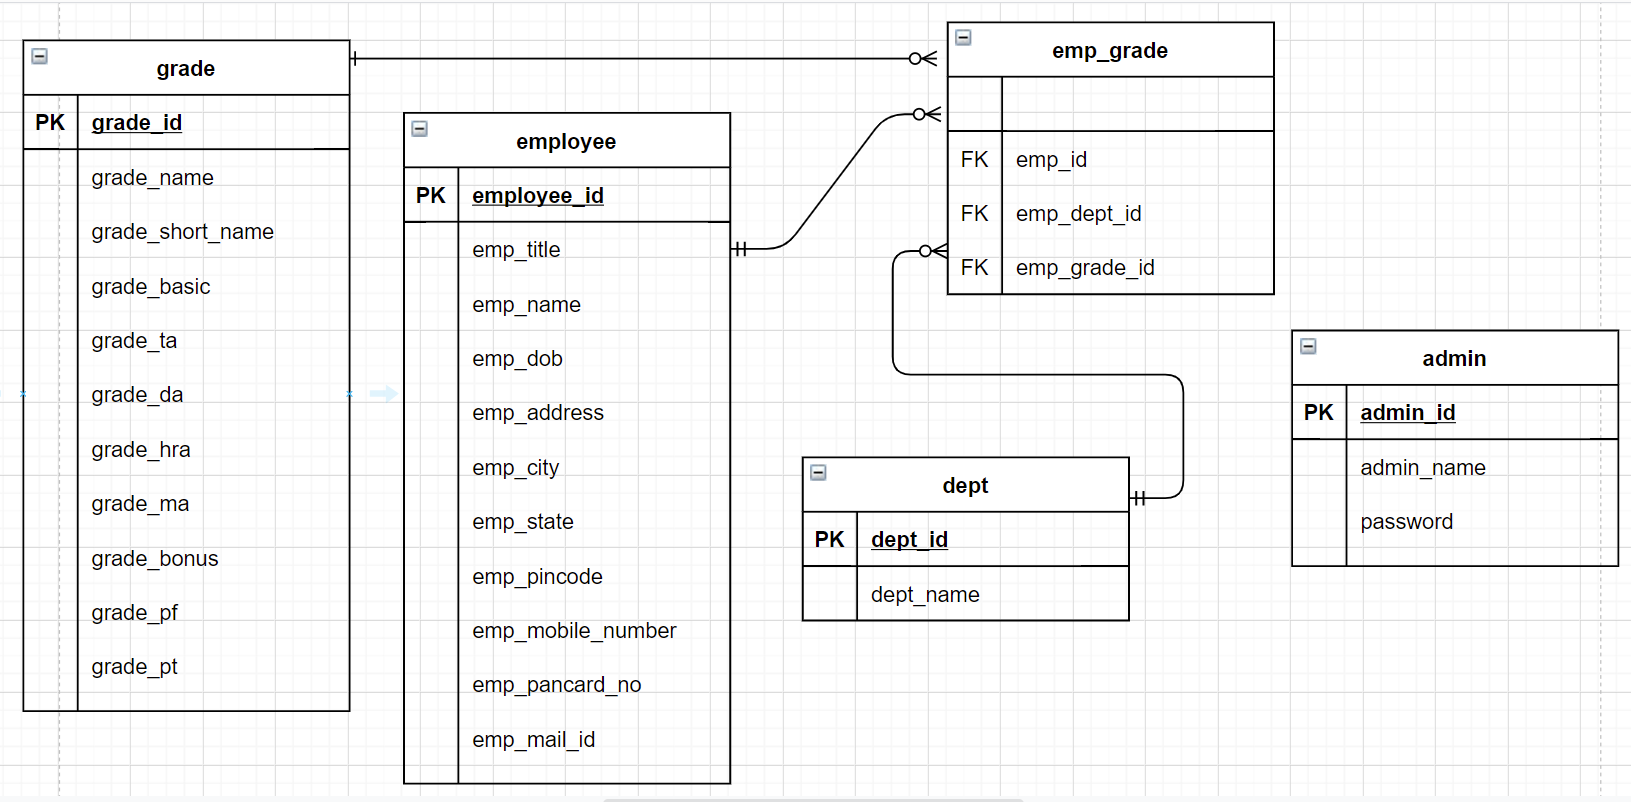
\includegraphics[width = \columnwidth]{er_diagram.png}
    \caption{Entity Relation Diagram}
    \label{fig:my_label}
\end{figure}
\noindent
From the ER diagram, the attributes corresponding to each entity can be seen. The foreign and primary key constraints applied on the tables have been highlighted as well. ( PK = Primary key, FK = Foreign key).


\newpage                            % Don't delete
\section{Source Code}               % Don't delete

\hl{Enclose the source code of your front end and back end separately.}

\newpage            % Don't delete
\section{Results}   % Don't delete

\hl{Enclose the snapshots of your results.}

\begin{figure}[h!]
    \centering
    %\includegraphics[width = \columnwidth]{output.png} % Here output.png is the file name of your snapshot. So, change only output.png with your file name and \caption{} to give some name. Don't touch other lines between \begin{figure} and \end{figure}
    %\caption{Factorial of a input number}
\end{figure}

\newpage
\section{References:}
\begin{enumerate}
    \item http://services.lovelycoding.org/hotel-management-system/
    \item https://1000projects.org/hotel-management-system-project.html
\end{enumerate}


\begin{center}
    \textbf{**** END ****}
\end{center}

\end{document}
